\documentclass[DIV=21,paper=A5,fontsize=10pt,twopage]{scrartcl}
%\documentclass[DIV=21,paper=20cm:20cm,9pt]{scrartcl}
\def\spal{2}
\setlength{\columnseprule}{0.4pt} % line between column
\usepackage{standalone}
\usepackage{titlesec}
\usepackage{multicol}
\usepackage{lettrine}

\usepackage{yfonts}\usepackage{soul}
\usepackage[dvipsnames]{xcolor}

\usepackage{tikz}
\usetikzlibrary{decorations.text}
%\usepackage{libertineotf}


\usepackage{dingbat}
\usepackage{collect}
\usepackage{ulem}
\definecollection{trs}

%\usepackage[hidelinks]{hyperref}
\usepackage{cleveref}
%\hypersetup{
%pdftitle={Pentagame Regulae Rules Regeln Regles},
%pdfsubject={Pentagame Rules in Many Languages},
%pdfauthor={Jan Suchanek et al.},
%pdfkeywords={Pentagame board game rules explained latin english german deutsch latine francais russian chinese spanish espaniol}
%}



%\usepackage{tikzpeople}

\usepackage{mdframed}
\usepackage{polyglossia}
\usepackage{xeCJK}
\providecommand{\chapterformat}{}
\setmainlanguage{english}
\setotherlanguages{french,ngerman,latin,italian,hindi,bahasai,farsi,russian,greek,spanish,georgian,swedish,polish,danish,turkish,dutch,finnish,arabic}

\DeclareTextCommandDefault{\cyrdash}{\hbox to.8em{---}~}

\makeatletter
\newcommand\footnoteref[1]{\protected@xdef\@thefnmark{\ref{#1}}\@footnotemark}
\makeatother

\newCJKfontfamily{\tradChinesefont}{AR PL UKai HK}[BoldFont=Noto Sans CJK TC Bold]
\newCJKfontfamily{\japanesefont}{Noto Sans CJK JP}
% Plain fontspec fonts (as opposed to the xeCJK \newCJKfontfamily ones above)
% used only for the CJK entries in the table of contents. xeCJK's automatic
% CJK/Latin font switching (and \newCJKfontfamily-declared fonts) stop working
% once \tableofcontents replays two or more polyglossia \selectlanguage
% switches from the .toc file, so the ToC lines need a font command that
% does not depend on xeCJK's script-detection state.
\newfontfamily\tocTradChinesefont{AR PL UKai HK}
\newfontfamily\tocJapanesefont{Noto Sans CJK JP}
\newfontfamily\tocSimpChinesefont{Noto Sans CJK SC}
\newfontfamily\arabicfont[Script=Arabic]{Amiri}
\newfontfamily\arabicfontsf[Script=Arabic]{Amiri}
\newfontfamily\georgianfont[Script=Georgian]{FreeSerif}
\newfontfamily\hindifont[Script=Devanagari]{Noto Sans Devanagari}
\usepackage{setspace}

\usepackage{marvosym} % for heart shape
\usepackage{microtype}
\usepackage{shapepar}

% does not seem necessary at all?!
%\setmainfont{FreeSans}
\setsansfont{FreeSans}
\setmainfont{FreeSerif}
\setCJKmainfont{Noto Sans CJK SC}
\setCJKsansfont{Noto Sans CJK SC}

%\setmonofont{FreeSerif}

\usepackage{tikz}
\raggedbottom
\raggedcolumns
\clubpenalty = 10000
\widowpenalty = 10000
\displaywidowpenalty = 10000

\newcommand{\noun}[1]{\textsc{#1}}

\newcounter{oldpage}

\makeatletter
\renewcommand\paragraph{%
\@startsection{paragraph}{4}%
{\z@}{1ex\@plus 1ex \@minus .2ex}%
{0.2ex \@plus .2ex}%
  {\sffamily\normalsize\bfseries}%
 }
 \makeatother

%%% Document specific commands

\newcommand{\myskip}{\smallskip}
\newcommand{\headline}{{\LARGE{}Pentagame}}
\newcommand{\tocent}{}
\newcommand{\tocline}{}
\newcommand{\translator}{}
\newcommand{\general}{}
\newcommand{\choosext}{}
\newcommand{\choosex}{}
\newcommand{\setupt}{}
\newcommand{\setup}{}
\newcommand{\objectivet}{}
\newcommand{\objective}{}
\newcommand{\rulest}{}
\newcommand{\rules}{}
\newcommand{\website}{\textsf{\textbf{pentagame.org}}}
\newcommand{\myhead}{\begin{centering}{\sffamily\Large{\textbf\headline}}\end{centering}}


%%% THE ACTUAL LAYOUT %%%
\newcommand{\layout}{
    \begin{mdframed}
        \centering {{{\Large{\textbf{\tocent}}}}}
    \end{mdframed}
    \addcontentsline{toc}{section}{\tocline}
    \begin{multicols}{2}
    \general
    \paragraph*{\choosext}
    \choosex
    \paragraph*{\setupt}
    \setup
    \paragraph*{\objectivet}
    \objective
    \paragraph*{\rulest}
    \rules
    \par
    %\hfill{\footnotesize{(\translator)}}
    \end{multicols}
    \newpage
}

%%% Arabic Layout
\newcommand{\layoutara}{
    \begin{mdframed}
        \centering {{{\Large{\textbf{\tocent}}}}}
    \end{mdframed}
    \addcontentsline{toc}{section}{\tocline}
    \begin{multicols}{2}
    %\RLmulticolcolumns
    \RTLmulticolcolumns  %% Only this works properly with the bidi package
        \general\par
        \medskip\uline{\textbf{\choosext}}\par\smallskip
        \choosex\par
        \medskip\uline{\textbf{\setupt}}\par\smallskip
        \setup\par
        \medskip\uline{\textbf{\objectivet}}\par\smallskip
        \objective\par
        \medskip\uline{\textbf{\rulest}}\par\smallskip
        \rules
    %\hfill{\footnotesize{(\translator)}}
    \end{multicols}
    \newpage
}


%% FRAKTUR LAYOUT

\newcommand{\layoutfrak}{
    %\renewcommand{\frakdefault}{ysmfrak}
    \frakfamily\fraklines
    \large
    \begin{mdframed}
        \centering {{{\Large{\textswab{\tocent}}}}}
    \end{mdframed}
    \addcontentsline{toc}{section}{\tocline}
    \begin{multicols}{2}
        \general\par
        \medskip\textswab{Poppen}\par\smallskip  % frak seems not to work with a command!
        \choosex\par
        \medskip\textswab{Opbuu}\par\smallskip
        \setup\par
        \medskip\textswab{Teel vun de Speel}\par\smallskip
        \objective\par
        \medskip\textswab{Regelwark}\par\smallskip
        \rules
    %\hfill{\footnotesize{(\translator)}}
    \end{multicols}
    \newpage
}

\setlength{\parskip}{0ex}
\setlength{\parindent}{0cm}


\title{\so{PENTAGAME}}
%\subtitle{The diceless pentagram shaped board game}
\author{Jan Suchanek}
\date{}
%\publishers{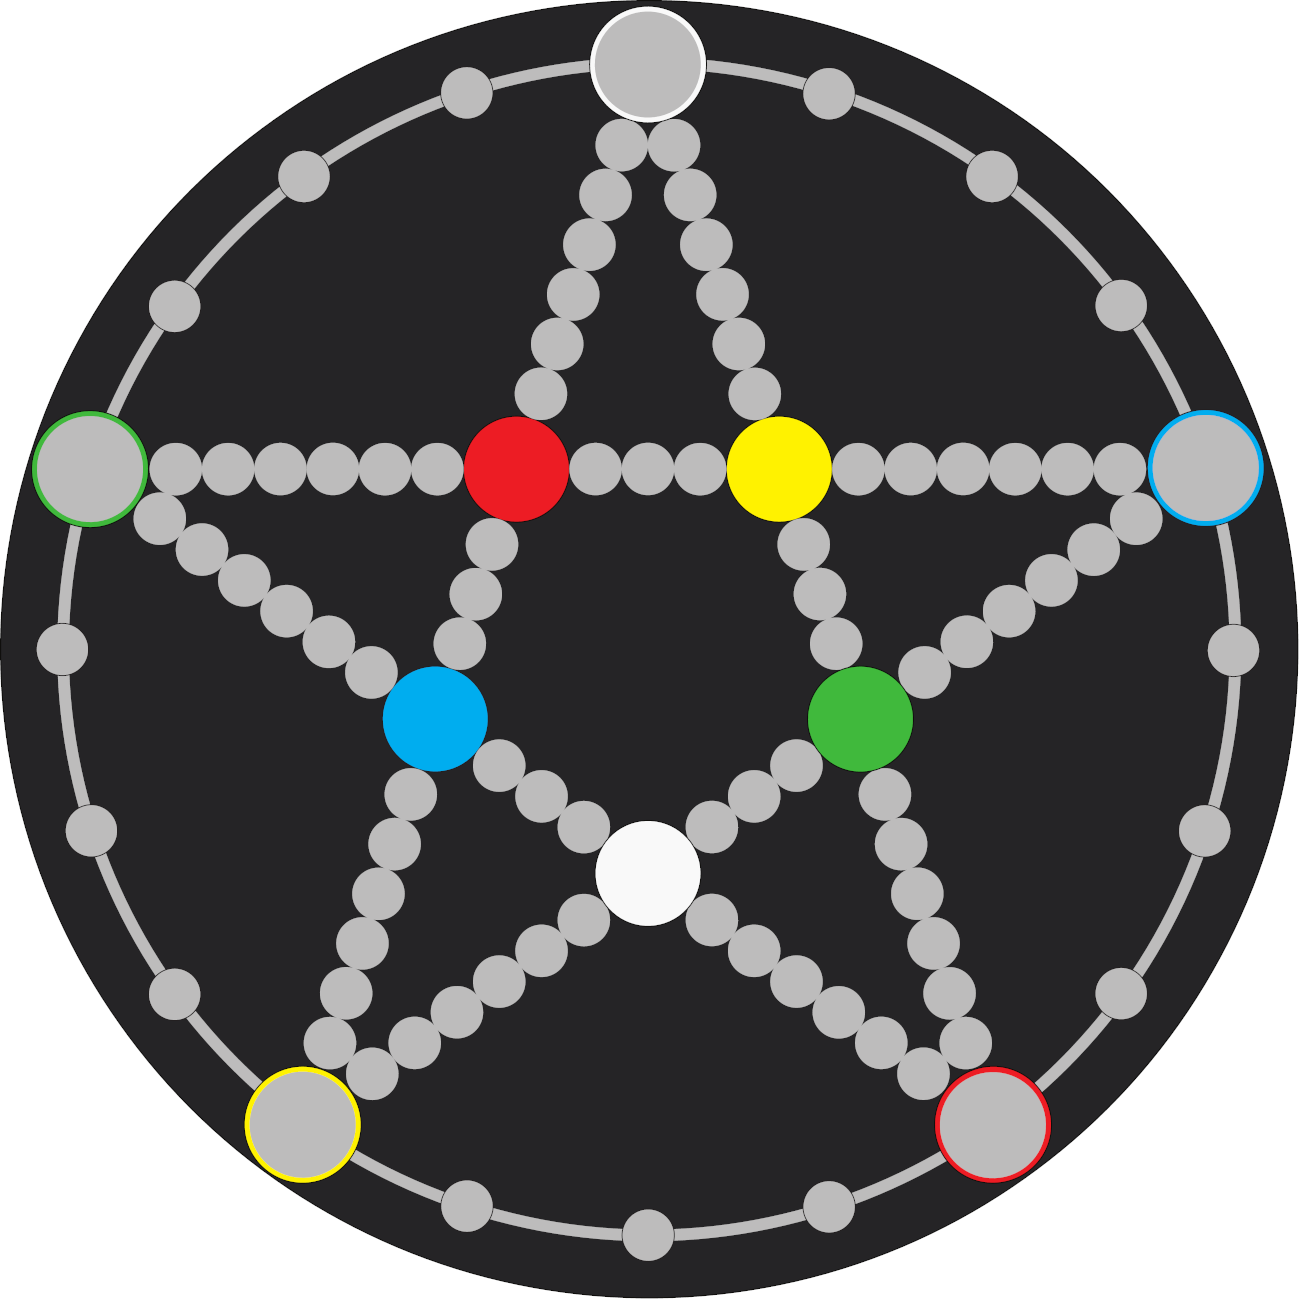
\includegraphics[width=0.382\textwidth]{Pentagame-board-nob.png}}
%\publishers{\input{pentagameinblue.tex}}


%% Actual Document. Calling the content first, then printing the same layout.

\begin{document}

\maketitle
\thispagestyle{empty}

\vfill

\begingroup
\raggedright
\hyphenpenalty=10000
\exhyphenpenalty=10000
\setlength\columnsep{28pt}
\makeatletter
\renewcommand\tableofcontents{%
    \@starttoc{toc}%
}
\renewcommand{\l@section}[2]{%
    \par\noindent #1\dotfill #2\par\smallskip
}
\makeatother
\begin{multicols}{2}
\tableofcontents
\end{multicols}
\endgroup

\vfill
\setlength\columnsep{10pt}

%\newpage\thispagestyle{empty}
%\emph{`Eon is a child at play, moving counters; the kingdom is a child's.'}

%\hfill ---\noun{Heraclitus}

%\hfill B52DK

%\vspace{25ex}
%\begin{center}
%    \input{pentalpha.tex}
%\end{center}
%\vfill

%Berlin $2020$

\newpage

%1. doppelseite
\begin{otherlanguage}{latin}
    \renewcommand{\headline}{Penta$\cdot$ludus - Latine}
\renewcommand{\tocent}{Latine}
\renewcommand{\tocline}{Regulae Latinae}
\renewcommand{\translator}{Dr.~J\"org Grimm, JS}
\renewcommand{\general}{ 
    \lettrine[lines=3]{L}{udus}
    mirabilis atque explicabilis velox. 
    Duo lusores ludent tertiam partem horae, tres aut quattuor ludent horam. 
    
    Alea non opus est. 
    Aptus lusoribus a quinque annis.
    Tabula pentagrammiforma, quattuor cohortes quinorum peditum coloratorum, quina impedimenta nigra et cana Penta\-ludum componunt.  Fit Ioh.~\noun{Aridus.}
}
\renewcommand{\choosext}{Cohortes}
\renewcommand{\choosex}{
    Lusor quisque agit pedites quinos, quibus est eadem forma, sed sunt diversi coloris. 
    
    Sic tua cohors peditem caeruleum, peditem rubrum et sequentes continet.
}

\renewcommand{\setupt}{Dispositio} 
\renewcommand{\setup}{ 
    In quinque nodis positis in circulo, qui circumvenit pentagramma, ponite pedites eiusdem coloris: pedites albos in nodo albo, caeruleos
    in nodo caeruleo, et sequentes. 
    
    Praeter illa decem aedicula quae nodos formant, existunt alia octoginta aedicula in viis, ubi pedites in ludo etiam possunt collocari. 
    
    Sunt etiam impedimenta nigra et im\-pe\-di\-men\-ta cana. 
    Impedimenta nigra ponite in nodis centri. In centro retinete impedimenta cana. 
}

\renewcommand{\objectivet}{Propositum} 
\renewcommand{\objective}{ 
    Destinatio per unum quemque peditem, qui occupat nodum externi circuli, est nodus eiusdem coloris in interno pentagrammatis. 
    Albo est eundum ad album, rubro ad rubrum, et sequentes. 
    
    Lusor victor qui duxit tres pedites ad nodum aequi coloris.
}

\renewcommand{\rulest}{Regulae } 
\renewcommand{\rules}{ 
    Duc peditum tuorum unum in quamvis directionem sequens aut viam circuli aut vias stellae, quoad per regulas potes occupare aediculum. 

    \myskip
    
    In quolibet aediculo libero, ubi  duae lineae conveniunt, tibi licet de via recta declinare sine retentione. 
    
    \myskip
    
    At numquam tibi licet transcendere nec impedimenta nec pedites alios.
    
    \myskip
    
    Potes vero ingredi in aediculum occupatum:
    
    \myskip
    
    Si ibi stat impedimentum nigrum, id pone in aediculo libero ad libitum. 
    
    Si ibi iam stat pedes alius, pedites positiones suas mutare debent.
    
    Si ibi sunt plures pedites (non potest fieri, nisi initio ludi), elige unum mutandum.
    
    \myskip
    
    Ita potes etiam mutare positiones duorum peditum tuorum.
    
    \myskip
    
    Eundem motum non licet iterum.
    
    \myskip
    
    Pedes progressus ad finem ludo abit. Colloca in centrum.
    
    Accipe inde impedimentum canum et colloca in aediculo libero, quoad tibi paret. 
    
    \myskip
    
    Si captas tale impedimentum canum, recolloca in centrum.
    
    \myskip
    
    Si non satis impedimenta cana, in ludo recolloca tale.
    
    \myskip
    
    Si alius lusor ad finem posivit peditem tuum, tibi is deinde removendus est.
    
    \myskip
    
    Orbis ultimus perficiatur.
}

    \layout 
\end{otherlanguage}

\begin{otherlanguage}{italian}
    \renewcommand{\headline}{Penta$\cdot$gioco - Italiano}
\renewcommand{\tocent}{Italiano}
\renewcommand{\tocline}{Regole in italiano}
\renewcommand{\translator}{Bozza di Claude, in attesa di revisione}
\renewcommand{\general}{
\lettrine[lines=3]{U}{n} gioco che si può spiegare in un minuto ma che rimane avvincente per anni.

In due si gioca in appena 20 minuti. In tre o quattro si può arrivare fino a 90 minuti.

Non servono dadi. Adatto a tutti dai 5 anni in su.

Nella scatola: 4$\times$5 pedine colorate, 5 blocchi neri e 5 grigi, il tabellone.
}

\renewcommand{\choosext}{Scegli le tue pedine}
\renewcommand{\choosex}{
Ogni giocatore ha cinque pedine. Nella scatola c'è una squadra di pedine per ogni giocatore.

Hai una pedina blu, una rossa, una bianca, una verde e una gialla.

Iniziano ai cinque angoli del tabellone corrispondenti al loro colore.

Vogliono raggiungere le grandi fermate al centro, dove escono dal gioco.
}

\renewcommand{\setupt}{Preparazione}
\renewcommand{\setup}{
Metti le tue pedine sui grandi angoli dell'anello corrispondenti al loro colore: la pedina bianca nell'angolo bianco dell'anello, la pedina blu nell'angolo blu dell'anello, e così via.

Metti i blocchi neri sui cinque incroci al centro del tabellone.

Lascia i blocchi grigi al centro per dopo.
}

\renewcommand{\objectivet}{Obiettivo}
\renewcommand{\objective}{
Le pedine bianche vogliono andare all'incrocio bianco al centro, quelle blu all'incrocio blu, e così via. La destinazione è sempre la grande fermata colorata al centro del pentagono, opposta al punto di partenza.

Sii il primo a spostare \emph{tre} pedine nelle loro destinazioni per vincere.
}

\renewcommand{\rulest}{Le regole}
\renewcommand{\rules}{
Sposta una qualsiasi delle tue pedine sulla stella o sull'anello, in qualsiasi direzione, per quanto vuoi.

Puoi girare in qualsiasi angolo o incrocio libero senza fermarti.

Non puoi mai saltare\textemdash né sopra i blocchi, né sopra altre pedine.

\myskip

Ma puoi muoverti \emph{su} una fermata occupata:

\myskip

Se così facendo catturi un blocco nero, mettilo su una fermata libera a tua scelta.

Se così facendo ti sposti su una fermata con un'altra pedina, scambia la posizione con essa.

\myskip

Puoi scambiare le posizioni di due delle tue pedine.

Se ti sposti su una fermata con più pedine, scegline una con cui scambiare.

\myskip

Non fare due volte di seguito la stessa identica mossa.

\myskip

Una pedina che ha raggiunto la sua destinazione viene tolta dal gioco. Mettila al centro del tabellone. Poi prendi uno dei blocchi grigi e mettilo su una fermata libera a tua scelta.

Se catturi un blocco grigio in questo modo, toglilo di nuovo dal tabellone.

Se finisci i blocchi grigi, sposta uno di quelli già in gioco.

\myskip

Se un altro giocatore ti ha spostato sulla tua meta, devi uscire non appena arriva il tuo turno.

\myskip

L'ultimo giro si gioca fino alla fine.
}

    \layout 
\end{otherlanguage}

\input{english.tex}%% English 
\layout

\begingroup
% \hyphenpenalty=10000
% \exhyphenpenalty=10000
{\small
% DRAFT ChiShona (Shona) translation.
% This is a from-scratch, research-assisted draft, not a native-speaker
% translation. Shona's noun-class agreement system is complex; please have
% a fluent ChiShona speaker check it before publishing.
\renewcommand{\headline}{Pe\-nta$\cdot$mu\-ta\-mbo - Chi\-Sho\-na}
\renewcommand{\tocent}{Chi\-Sho\-na}
\renewcommand{\tocline}{Mi\-te\-mo mu\-Chi\-Sho\-na}
\renewcommand{\translator}{Sha\-ndu\-ro ye\-ku\-ta\-nga (AI), i\-no\-da kuo\-ngo\-ro\-rwa ne\-mu\-tau\-ri we\-chi\-zva\-rwa}
\renewcommand{\general}{
\lettrine[lines=3]{M}{u\-ta\-mbo} u\-no\-go\-na ku\-tsa\-na\-ngu\-rwa mu\-ka\-ti me\-mi\-ne\-ti i\-mwe, a\-si u\-no\-ra\-mba u\-chi\-fa\-dza va\-nhu kwe\-ma\-ko\-re ma\-zhi\-nji.

Va\-ta\-mbi va\-vi\-ri va\-no\-ta\-mba kwe\-ma\-mi\-ni\-tsi ma\-ku\-mi ma\-vi\-ri che\-te. Va\-ta\-tu ka\-na va\-na va\-nga\-to\-ra ku\-svi\-ka kwe\-ma\-mi\-ni\-tsi ma\-ku\-mi ma\-pfu\-mba\-mwe.

Ha\-pa\-na ma\-dhai\-si a\-no\-sha\-ndi\-swa. Mu\-ta\-mbo u\-yu wa\-ka\-ko\-dze\-ra mu\-nhu we\-se, ku\-bvi\-ra pa\-ze\-ra re\-ma\-ko\-re ma\-sha\-nu zvi\-chi\-kwi\-ra.

Mu\-bho\-ki\-si mu\-ne: zvi\-dho\-ri zvi\-na zvi\-ne ru\-va\-ra, zvi\-sha\-nu pa\-ne ri\-mwe ne\-ri\-mwe (4$\times$5), zvi\-dho\-ri zvi\-te\-ma zvi\-sha\-nu, zvi\-dho\-ri zvi\-pfu\-mbu zvi\-sha\-nu, u\-ye bho\-dhi re\-mu\-ta\-mbo.
}

\renewcommand{\choosext}{Sa\-ru\-dza zvi\-dho\-ri zva\-ko}
\renewcommand{\choosex}{
Mu\-ta\-mbi mu\-mwe no\-mu\-mwe a\-ne zvi\-dho\-ri zvi\-sha\-nu. Mu\-bho\-ki\-si mu\-ne bo\-ka re\-zvi\-dho\-ri ri\-mwe pa\-mu\-ta\-mbi.

U\-ne chi\-dho\-ri che\-bhu\-ruu, chi\-dho\-ri chi\-tsvu\-ku, chi\-dho\-ri chi\-che\-na, chi\-dho\-ri che\-gi\-ri\-ni ne\-chi\-dho\-ri che\-ye\-ro.

Zvi\-dho\-ri zvi\-no\-ta\-nga pa\-ma\-ko\-na ma\-sha\-nu e\-bho\-dhi, ko\-na i\-mwe nei\-mwe i\-ne ru\-va\-ra rwu\-noe\-nde\-ra\-na ne\-chi\-dho\-ri.

Zvi\-no\-da ku\-svi\-ka pa\-nzvi\-mbo hu\-ru dzi\-ri pa\-ka\-ti pe\-bho\-dhi. I\-pa\-po, zvi\-no\-bvi\-swa pa\-mu\-ta\-mbo.
}

\renewcommand{\setupt}{Ku\-ga\-dzi\-ri\-ra}
\renewcommand{\setup}{
I\-sa zvi\-dho\-ri zva\-ko pa\-ma\-ko\-na ma\-ku\-ru a\-ri pa\-de\-nde\-re\-dzwa, ko\-na i\-mwe nei\-mwe i\-chie\-nde\-ra\-na ne\-ru\-va\-ra rwe\-chi\-dho\-ri: chi\-dho\-ri chi\-che\-na pa\-ko\-na che\-na, chi\-dho\-ri che\-bhu\-ruu pa\-ko\-na bhu\-ruu, u\-ye zvi\-mwe zva\-ka\-da\-ro.

I\-sa zvi\-dho\-ri zvi\-te\-ma pa\-nzvi\-mbo sha\-nu dzi\-ri pa\-ka\-ti pe\-bho\-dhi, a\-po mi\-tsa\-ra i\-no\-sa\-nga\-na.

Che\-nge\-ta zvi\-dho\-ri zvi\-pfu\-mbu pa\-ka\-ti pe\-bho\-dhi; zvi\-cha\-sha\-ndi\-swa ga\-re ga\-re.
}

\renewcommand{\objectivet}{Chi\-na\-ngwa}
\renewcommand{\objective}{
Zvi\-dho\-ri zvi\-che\-na zvi\-no\-da ku\-svi\-ka pa\-nzvi\-mbo che\-na i\-ri pa\-ka\-ti, zve\-bhu\-ruu pa\-nzvi\-mbo ye\-bhu\-ruu, u\-ye zvi\-mwe zva\-ka\-da\-ro. Nzvi\-mbo i\-no\-di\-wa i\-no\-ga\-ra i\-ri nzvi\-mbo hu\-ru i\-ne ru\-va\-ra rwa\-ka\-fa\-na\-na, i\-ri pa\-ka\-ti pe\-pe\-nda\-go\-ni, mhi\-ri kwe\-nzvi\-mbo ye\-ku\-ta\-ngi\-ra.

Fa\-mbi\-sa \emph{zvi\-dho\-ri zvi\-ta\-tu} ku\-nzvi\-mbo dza\-zvo ku\-ti u\-ku\-nde.
}

\renewcommand{\rulest}{Mi\-te\-mo}
\renewcommand{\rules}{
Fa\-mbi\-sa chi\-mwe che\-zvi\-dho\-ri zva\-ko pa\-nye\-re\-dzi ka\-na pa\-de\-nde\-re\-dzwa, ku\-nzi\-ra i\-pi nei\-pi, ku\-svi\-ka pau\-no\-da.

U\-no\-go\-na ku\-te\-ndeu\-ka pa\-ko\-na i\-pi nei\-pi i\-si\-na chi\-nhu, ka\-na pa\-nzvi\-mbo i\-pi nei\-pi i\-no\-sa\-nga\-na ne\-mi\-tsa\-ra mi\-vi\-ri, u\-si\-nga\-mi\-ri.

\myskip

U\-sa\-to\-mbo\-da\-ri\-ka chi\-nhu -- ku\-nya\-nge zvi\-dho\-ri zvi\-te\-ma, ku\-nya\-nge zvi\-mwe zvi\-dho\-ri.

\myskip

A\-si u\-no\-go\-na ku\-fa\-mbi\-ra pa\-nzvi\-mbo i\-ne chi\-mwe chi\-nhu:

\myskip

Ka\-na wa\-fa\-mbi\-ra pa\-nzvi\-mbo i\-ne chi\-dho\-ri chi\-te\-ma, chi\-to\-re u\-chi\-chii\-sa pa\-nzvi\-mbo i\-pi nei\-pi i\-si\-na chi\-nhu, so\-ku\-da kwa\-ko.

Ka\-na wa\-fa\-mbi\-ra pa\-nzvi\-mbo i\-ne chi\-mwe chi\-dho\-ri, chi\-nja\-nai nzvi\-mbo na\-cho.

\myskip

U\-no\-go\-na ku\-chi\-nja\-ni\-sa nzvi\-mbo dze\-zvi\-dho\-ri zva\-ko zvi\-vi\-ri.

Ka\-na wa\-fa\-mbi\-ra pa\-nzvi\-mbo i\-ne zvi\-dho\-ri zva\-ka\-wa\-nda, sa\-ru\-dza chi\-mwe ku\-ti mu\-chi\-nja\-ne nzvi\-mbo.

\myskip

U\-sai\-te mu\-fa\-mbi\-ro mu\-mwe che\-te ka\-vi\-ri zvi\-chi\-te\-ve\-dza\-na.

\myskip

Chi\-dho\-ri cha\-svi\-ka kwa\-chi\-no\-da chi\-no\-bvi\-swa pa\-bho\-dhi. Chii\-se pa\-ka\-ti pe\-bho\-dhi. I\-pa\-po to\-ra chi\-mwe che\-zvi\-dho\-ri zvi\-pfu\-mbu, u\-chi\-chii\-sa pa\-nzvi\-mbo i\-si\-na chi\-nhu, so\-ku\-da kwa\-ko.

Ka\-na wa\-fa\-mbi\-ra pa\-ne chi\-dho\-ri chi\-pfu\-mbu cha\-ka\-da\-ro, chi\-bvi\-se pa\-bho\-dhi zva\-ka\-re.

Ka\-na zvi\-dho\-ri zvi\-pfu\-mbu zva\-pe\-ra, chi\-nja\-ni\-sa chi\-mwe che\-zvi\-ri ku\-ta\-mba mu\-mu\-ta\-mbo.

\myskip

Ka\-na mu\-mwe mu\-ta\-mbi a\-ka\-ku\-fa\-mbi\-sa ku\-svi\-ka kwau\-no\-da, u\-no\-fa\-ni\-ra ku\-zvi\-bvi\-sa pa\-bho\-dhi pa\-mu\-ka\-na wa\-ko u\-no\-te\-ve\-ra.

\myskip

Da\-nho ro\-ku\-pe\-dzi\-si\-ra ri\-no\-ta\-mba ku\-svi\-ka ra\-pe\-ra.
}

\layout
}
\endgroup


%2. doppelseite
\begin{otherlanguage}{french}
    \input{francais.tex}
    \layout
\end{otherlanguage}

\begin{otherlanguage}{spanish}
    
\renewcommand{\headline}{Penta$\cdot$juego - Español}	
\renewcommand{\tocent}{Español}	
\renewcommand{\tocline}{Reglas en español}
\renewcommand{\translator}{Juan José Bravo / Carlos Ayon}	
\renewcommand{\general}{
    \lettrine[lines=3]{U}{n}
    juego que se explica en un minuto, pero que sigue fascinándote durante años. 
    Una partida entre dos jugadores puede llevarte 20 minutos. Tres o cuatro jugadores pueden tardar hasta 90 minutos.	
    Se juega sin dados. Apto para todos, a partir de los cinco años.	
    En la caja: 4 x 5 figuras de colores, 5 bloques negros, 5 grises y un tablero.	
}		
	
\renewcommand{\choosext}{Elije tus figuras}	
\renewcommand{\choosex}{	
En la caja hay un grupo de figuras por jugador. Cada equipo está compuesto por cinco figuras; una azul, una roja, una blanca, una verde  y una amarilla.	
Las figuras se colocan en los círculos exteriores de los colores correspondientes:
Ellas tendrán que llegar a la meta situada en el medio del tablero. 	
}	

\renewcommand{\setupt}{Instalación}	
\renewcommand{\setup}{	
Disponed vuestras figuras sobre los círculos exteriores en sus colores correspondientes: 
la figura blanca en el círculo exterior blanco, la azul en círculo exterior azul, etc.	
	
Dispón los bloques negros en los cinco círculos interiores en el medio del tablero.
Coloca los bloques grises en el centro del tablero.	
}	
	
\renewcommand{\objectivet}{Objetivo}	
\renewcommand{\objective}{	
Las figuras blancas deben alcanzar los círculos interiores blancos, las figuras azules los círculos interiores azules, etc.	
El destino es siempre el gran círculo central, del color correspondiente a la figura, en el medio del pentágono opuesto al punto de partida.	
	
Coloca \emph{tres} de tus cinco peones en los círculos de colores correspondientes para ganar.
}	
	
\renewcommand{\rulest}{Reglas del juego}	
\renewcommand{\rules}{	
Mueve la figura de tu elección sobre el tablero de juego sin importar la dirección, tan lejos como quieras.	
	
Puedes girar en cualquier esquina o intersección libres, sin detenerte.	
	
No podrás saltar sobre ningún bloque o figura, pero podrás colocarte en un círculo  ocupado:	
	
\myskip	
	
Si caes en un círculo ocupado por un bloque negro, tómalo y colócalo en cualquier espacio libre de tu elección.	
	
Si caes en un círculo ocupado por otra figura, intercambia tu lugar anterior con ella.	
	
	
Puedes cambiar de posición entre dos peones de tu propio equipo. 	


Si caes en una casilla ocupada por varias figuras, puedes elegir una de ellas e intercambiar de lugar.	

\myskip	
	
No puedes hacer el mismo movimiento dos veces seguidas.	

\myskip
	
Cuando una figura llega a su meta, es retirada del juego. Se le coloca en el centro del tablero y se toma un peón gris que podrás colocar en cualquier círculo libre de tu elección.
	
\myskip		
	
Si caes en un lugar ocupado por un bloque gris, este será retirado del juego nuevamente.	

Si se acaban los bloques grises, mueve uno de los que ya están en juego.

\myskip	

Si otro jugador ha movido una de tus figuras a su meta, debes retirarla en cuanto sea tu turno.

\myskip	

La última ronda se juega hasta el final.
	
% El primer jugador que consiga retirar tres de sus figuras ganará la partida.%
}


    \layout
\end{otherlanguage}

%3. doppelseite
\begin{otherlanguage}{ngerman}
    \input{deutsch.tex}
    \layout
\end{otherlanguage}

\begin{otherlanguage}{german} % platt
    \input{platt.tex}
    \layout%frak 
\end{otherlanguage}

%4. doppelseite
\begin{otherlanguage}{dutch}
\input{nederlands.tex}
\layout
\end{otherlanguage}

\begin{otherlanguage}{danish}
\input{danish.tex}
\layout
\end{otherlanguage}

%5. doppelseite - HEFTMITTE
\begin{otherlanguage}{polish}
    \input{polski.tex}
    \layout
\end{otherlanguage}

\begin{otherlanguage}{russian}
    \input{russian.tex}
    \raggedright
    {\layout}
\end{otherlanguage}

%6. doppelseite
\begin{otherlanguage}{swedish}
    \input{swedish.tex}
    \layout
\end{otherlanguage}

\begin{otherlanguage}{finnish}
    {\small
    \input{finnish.tex}
    \layout
    }
\end{otherlanguage}

%7. doppelseite
\begin{otherlanguage}{georgian}
    \renewcommand{\headline}{პენტა $\cdot$ გამა - 
ქართული}
\renewcommand{\tocent}{ქართული}
\renewcommand{\tocline}{წესები ქართულად}
\renewcommand{\translator}{Irakli Sakvarelidze}
\renewcommand{\general}{
    \lettrine[lines=3,loversize=0.7]{თ}{ამაში,} რომელიც მარტივი და ამავე დროს მიმზიდველია. 
    თამაშის ხანგრძლივობა გრძელდება 20წ.-დან 90წ.-მდე, რაც განისაზღვრება იმის და მიხედვით თუ რამდენი მოთამაშე მონაწილეობს.
    
    ყუთში მოთავსებულია, სათამაშო დაფასთან ერთდ 4$\times$5 სხვადახვა ფერის ფიგურები, 5 შავი და 5
    სერი.
}

\renewcommand{\choosext}{ფიგურების არჩევა}
\renewcommand{\choosex}{
ყოველი მოთამაშე იღებს 5 სხვადასხვა ფერის, მსგავსი ფორმის, ფიგურებს. 

ფიგურები სტარტს იღებენ დიდ წრეზე განთავსებული 5 ქიმერიდან. 

მათი მოვალეობაა, მიაღწიონ ცენტრალურ უბანს.

}
\renewcommand{\setupt}{მომზადება}
\renewcommand{\setup}{
დაალაგეთ ფიგურები ფერების მიხედვით, წრიულად ქიმებზე. 

შავი ფიგურები დაალაგეთ ცენტრში წრიულად გადამკვეთ ხაზებთან. 

სერი ფიგურები კი მოათავსეთ ცენტრში, ისინი გამოგვადგება შემდგომ.
}

\renewcommand{\objectivet}{მიზანი}
\renewcommand{\objective}{
იგებს ის ვინც პირველი გადაადგილებს სამ ფიგურას ფერების შესაბამის უჯრებში ხაზების გადაკვეთის წერტილებში. 

ამიტომ, იყავი პირველი.
}

\renewcommand{\rulest}{წესები}
\renewcommand{\rules}{

მოთამაშეს შეუძლია მოთამაშის ნებისმიერი ფიგურა გადაადგილოს ნებისმიერ დისტანციაზე წრიულად ან გადაკვეთის წერტილებში. 

სვლა შეგიძლია გააგრძელო იმ შემთხვევაში თუ წინ ფიგურა არ გხვდება. გადახტომა არ შეიძლება. 

თუ შავი ფიგურა შეგხვდა გადაადგილე ნებისმიერ ცარიელ უჯრაში. 

\myskip

თუ გადამკვეტ უჯრაში მოწინააღმდეგის ფიგურაა შეგხვდა დაბრკოლებად, გაუცვალე ადგილი. 

\myskip

თუ მიადეგით ადგილს სადაც რამოდენიმე მეტოქის ფიგურაა თავმოყრილი, ჩაანაცვლე ერთ-ერთი მათგანით. 

არ შეიძლება ერთი და იგივე სვლის ორჯერ გამეორება. 

\myskip

ფიგურა რომელიც მიაღწევს დანიშნულების ადგილს გადის თამაშიდან და მის მაგივრად, მოთამაშე იღებს სერ ფიგურას, რომლის მოთავსებაც შეიძლება ნებისმიერ თავისუფალ ადგილას. 

თუ ისეთ ადგილას მოხვდი, სადაც სერი ფიგურაა, ის მოაშორე დაფიდან.

თუ სერი ფიგურები აღარ დარჩა, გადაანაცვლე ერთ-ერთი უკვე დადებული ფიგურა.

\myskip
თუ მეორე მოთამაშემ შენი მიზნისკენ გადაგაადგილა, შენც უნდა გადახვიდე, სანამ შენი სვლაა!

\myskip
ბოლო ტური ბოლომდე ითამაშა.
}

    \raggedright
    {\layout}
\end{otherlanguage}

\begin{otherlanguage}{greek}
    \renewcommand{\headline}{Πέντε$\cdot$παιχνίδι - Eλληνικά}
\renewcommand{\tocent}{Eλληνικά}
\renewcommand{\tocline}{Κανόνες στα ελληνικά}
\renewcommand{\translator}{Athanasios Kostopoulos}
\renewcommand{\general}{
\lettrine[lines=3]{E}{να} παιχνίδι που μπορεί να εξηγηθεί σε ένα λεπτό αλλά παραμένει
συναρπαστικό για χρόνια.

Μια παρτίδα δύο παικτών διαρκεί μόλις 20 λεπτά. Μια παρτίδα
τριών ή τεσσάρων παικτών μπορεί να διαρκέσει ως 90 λεπτά.

Το παιχνίδι δεν χρησιμοποιεί ζάρια και είναι κατάλληλο για όλες τις
ηλικίες από 5 ετών και πάνω. 
%Ο σχεδιαστης του παιχνιδιου ειναι ο Jan \noun{Suchanek.}

Στο κουτί θα βρείτε: 4$\times$5 έγχρωμες φιγούρες, 5 μαύρα και
5 γκρίζα τουβλάκια, καθώς και το ταμπλό παιχνιδιού.
}

\renewcommand{\choosext}{Επιλογή φιγούρων}
\renewcommand{\choosex}{
Κάθε παίκτης έχει πέντε φιγούρες. Υπάρχει μία ομάδα φιγούρων ανά παίκτη στο κουτί.
%Μια ομαδα εχει ασπρα μαλλια, μια ομαδα μαυρα, μια ξανθα και μια ειναι φαλακρη.

%Οι παικτες πρεπει να διαλεξουν την ομαδα με την οποια μοιαζουν περισσοτερο.

Ο κάθε παίκτης έχει μία μπλε, μία κόκκινη, μία λευκή, μία πράσινη
και μία κίτρινη φιγούρα.

Αρχίζουν στις πέντε γωνίες του ταμπλό, ανάλογα με το χρώμα τους.

Ο στόχος είναι να φτάσουν στις μεγάλες στάσεις στο κέντρο του ταμπλό.

}
\renewcommand{\setupt}{Στήσιμο}
\renewcommand{\setup}{
Τοποθετήστε τις φιγούρες σας στις μεγάλες γωνίες του δακτυλίου, ανάλογα με το χρώμα τους:
η λευκή φιγούρα στη λευκή γωνία, η μπλε φιγούρα στην μπλε γωνία, κ.ο.κ.

Τοποθετήστε τα μαύρα τουβλάκια στις πέντε διασταυρώσεις στο μέσο του ταμπλό.

Αφήστε τα γκρίζα τουβλάκια στη μέση του ταμπλό για μετέπειτα χρήση. 
}

\renewcommand{\objectivet}{Στόχος παιχνιδιού}
\renewcommand{\objective}{
Οι λευκές φιγούρες θέλουν να πάνε στη λευκή διασταύρωση στο κέντρο,
οι μπλε φιγούρες στην μπλε, κ.ο.κ. Ο προορισμός είναι πάντα η μεγάλη,
έγχρωμη στάση στο μεσαίο πεντάγωνο, απέναντι από το σημείο εκκίνησης.

Ο πρώτος παίκτης που θα τοποθετήσει \emph{τρία} κομμάτια στον προορισμό τους, κερδίζει.
}

\renewcommand{\rulest}{Κανόνες παιχνιδιού}
\renewcommand{\rules}{
Μετακινήστε οποιαδήποτε από τις φιγούρες σας στο άστρο ή στο δακτύλιο, σε κάθε
κατεύθυνση, όσο θέλετε.

Μπορείτε να στρίψετε σε κάθε ελεύθερη γωνία ή διασταύρωση χωρίς να σταματήσετε.

Ποτέ δεν μπορείτε να πηδήξετε\textemdash ούτε πάνω από τουβλάκια, ούτε πάνω από φιγούρες. 

\myskip

Παρόλα αυτά, μπορείτε να μετακινηθείτε \emph{σε} μια κατειλημμένη θέση:

\myskip

Αν καταλάβετε θέση με μαύρο τουβλάκι, τοποθετήστε το σε μια ελεύθερη θέση της επιλογής σας.

Αν μετακινηθείτε σε θέση με μια άλλη φιγούρα, ανταλλάξτε θέσεις.
 
\myskip

Μπορείτε να ανταλλάξετε τις θέσεις δύο από τις φιγούρες σας.

Αν μετακινηθείτε σε θέση με πολλαπλές φιγούρες, διαλέξτε μία για ανταλλαγή θέσης.
 
\myskip 

Μην κάνετε την ίδια κίνηση δύο φορές συνεχόμενα.   

\myskip 

Μια φιγούρα που φτάνει στον προορισμό της αφαιρείται. Τοποθετήστε την στο κέντρο του ταμπλό. Αφού γίνει αυτό,
παίρνετε ένα από τα γκρίζα τουβλάκια και το τοποθετείτε σε ελεύθερη θέση της επιλογής σας.

\myskip

Αν πάτε σε θέση με γκρίζο τουβλάκι, το αφαιρείτε από το ταμπλό.

\myskip

Εάν μεταφερθείτε στον προορισμό σας από άλλο παίκτη, πρέπει να βγείτε από τη στροφή σας.

\myskip

Ο τελευταίος γύρος παίζεται μέχρι το τέλος.
}

    {\small
    \layout}
\end{otherlanguage}

\begin{otherlanguage}{turkish}
    \input{turkish}
    \layout
\end{otherlanguage}



\begin{otherlanguage}{hindi}
    \renewcommand{\headline}{Penta$\cdot$खेल - हिंदी}
\renewcommand{\tocent}{हिंदी}
\renewcommand{\tocline}{हिंदी में नियम}
\renewcommand{\translator}{क्लॉड द्वारा प्रारूप, समीक्षा आवश्यक}
\renewcommand{\general}{
एक ऐसा खेल जिसे एक मिनट में समझाया जा सकता है, लेकिन जो बरसों तक दिलचस्प बना रहता है।

दो खिलाड़ियों के बीच यह खेल सिर्फ़ 20 मिनट में ख़त्म हो जाता है। तीन या चार खिलाड़ियों के साथ इसमें 90 मिनट तक लग सकते हैं।

इसमें पासे का इस्तेमाल नहीं होता। यह 5 साल और उससे ऊपर के सभी लोगों के लिए उपयुक्त है।

डिब्बे में हैं: 4$\times$5 रंगीन गोटियाँ, 5 काले और 5 स्लेटी ब्लॉक, और बोर्ड।
}

\renewcommand{\choosext}{अपनी गोटियाँ चुनें}
\renewcommand{\choosex}{
हर खिलाड़ी के पास पांच गोटियाँ होती हैं। डिब्बे में हर खिलाड़ी के लिए गोटियों का एक सेट है।

आपके पास एक नीली, एक लाल, एक सफ़ेद, एक हरी और एक पीली गोटी होती है।

गोटियाँ बोर्ड के उन पांच कोनों से शुरू होती हैं जो उनके रंग से मेल खाते हैं।

वे बीच में मौजूद बड़े चौराहों तक पहुंचना चाहती हैं, जहाँ पहुँचकर वे खेल से बाहर हो जाती हैं।
}

\renewcommand{\setupt}{तैयारी}
\renewcommand{\setup}{
अपनी गोटियों को बाहरी घेरे के बड़े कोनों पर रखें, जो उनके रंग से मेल खाते हों: सफ़ेद गोटी को घेरे के सफ़ेद कोने पर, नीली गोटी को घेरे के नीले कोने पर, और इसी तरह बाकी गोटियों को भी रखें।

काले ब्लॉक बोर्ड के बीचोंबीच स्थित पांचों चौराहों पर रखें।

स्लेटी ब्लॉक बाद में इस्तेमाल करने के लिए बीच में रख दें।
}

\renewcommand{\objectivet}{लक्ष्य}
\renewcommand{\objective}{
सफ़ेद गोटियाँ बीच के सफ़ेद चौराहे तक जाना चाहती हैं, नीली गोटियाँ नीले चौराहे तक, और इसी तरह बाकी भी। मंज़िल हमेशा शुरुआती बिंदु के ठीक सामने, पंचभुज के केंद्र में स्थित बड़ा रंगीन चौराहा होती है।

जीतने के लिए सबसे पहले अपनी \textbf{तीन} गोटियाँ उनकी मंज़िल तक पहुँचाएँ।
}

\renewcommand{\rulest}{नियम}
\renewcommand{\rules}{
अपनी किसी भी गोटी को तारे की रेखाओं या बाहरी घेरे पर, किसी भी दिशा में, जितना चाहें उतना दूर तक चलाएँ।

आप बिना रुके किसी भी खाली कोने या चौराहे पर मुड़ सकते हैं।

आप कभी भी किसी के ऊपर से नहीं फांद सकते\textemdash न ब्लॉक के ऊपर से, न किसी और गोटी के ऊपर से।

\myskip

लेकिन आप किसी ऐसे स्थान पर \textbf{ज़रूर} जा सकते हैं जहाँ पहले से कुछ हो:

\myskip

अगर ऐसा करने से आप किसी काले ब्लॉक को हटाते हैं, तो उसे अपनी पसंद के किसी भी खाली स्थान पर रख दें।

अगर ऐसा करने से आप किसी और गोटी वाले स्थान पर पहुँचते हैं, तो उसके साथ अपनी जगह बदल लें।

\myskip

आप अपनी दो गोटियों की जगह आपस में बदल सकते हैं।

अगर आप ऐसे स्थान पर पहुँचें जहाँ कई गोटियाँ हों, तो उनमें से किसी एक के साथ जगह बदल लें।

\myskip

लगातार दो बार एक जैसी चाल न चलें।

\myskip

जो गोटी अपनी मंज़िल तक पहुँच जाए, उसे बोर्ड से हटाकर बीच में रख दें। इसके बाद स्लेटी ब्लॉकों में से एक उठाएँ और उसे अपनी पसंद के किसी खाली स्थान पर रख दें।

अगर आप इस तरह किसी स्लेटी ब्लॉक को हटाते हैं, तो उसे फिर से बोर्ड से हटा लें।

अगर स्लेटी ब्लॉक ख़त्म हो जाएँ, तो जो पहले से खेल में हैं उनमें से किसी एक को फिर से रखें।

\myskip

अगर किसी दूसरे खिलाड़ी ने आपकी किसी गोटी को उसकी मंज़िल तक पहुँचा दिया है, तो अपनी बारी आते ही आपको उसे हटाना होगा।

\myskip

आख़िरी दौर अंत तक खेला जाता है।
}

    \layout
\end{otherlanguage}

%{\tradChinesefont
\input{tradchinese.tex}
%\renewcommand{\tocent}{繁體中文}
{\large \layout}%}
\pagebreak
\input{simplechinese.tex}
{\large \layout}
\pagebreak
{\japanesefont
\renewcommand{\headline}{Penta$\cdot$ゲーム - 日本語}
\renewcommand{\tocent}{日本語}
\renewcommand{\tocline}{日本語のルール}
\renewcommand{\translator}{Claudeによる下訳、要確認}
\renewcommand{\general}{
1分で説明できるのに、何年経っても夢中になれるゲームです。

2人なら20分ほどで終わります。3人か4人なら90分ほどかかることもあります。

サイコロは使いません。5歳以上ならどなたでも楽しめます。

箱の中身:色のついた駒が4$\times$5個、黒いブロックが5個、グレーのブロックが5個、そしてボード。
}

\renewcommand{\choosext}{駒を選ぶ}
\renewcommand{\choosex}{
プレイヤーはそれぞれ5個の駒を持ちます。箱の中には、プレイヤー1人分の駒セットが入っています。

青、赤、白、緑、黄色の駒が1個ずつあります。

駒は、それぞれの色に対応するボードの隅からスタートし、中央にある大きな交点を目指します。到達すると、その駒は盤から取り除かれます。
}

\renewcommand{\setupt}{準備}
\renewcommand{\setup}{
それぞれの駒を、色が対応する外側の輪の大きな隅に置きます。白い駒は白い隅に、青い駒は青い隅に、というように置いていきます。

黒いブロックは、盤の中央にある5つの交点に置きます。

グレーのブロックは、後で使うので中央に置いておきます。
}

\renewcommand{\objectivet}{目的}
\renewcommand{\objective}{
白い駒は中央の白い交点を、青い駒は青い交点を目指します。目的地は常に、出発点の反対側にある、五角形の中心にある大きな色付きの交点です。

先に\emph{3個}の駒を目的地へ動かした人が勝ちです。
}

\renewcommand{\rulest}{ルール}
\renewcommand{\rules}{
自分の駒を1つ選び、星の線か外側の輪に沿って、好きな方向に好きなだけ動かします。

途中の空いている隅や交点では、止まらずに曲がることができます。

ブロックの上も、他の駒の上も、決して飛び越えることはできません。

\myskip

ただし、すでに駒やブロックがある場所へ進むことはできます:

\myskip

そうして黒いブロックのある場所に進んだ場合は、そのブロックを好きな空いている場所に置き直します。

そうして他の駒がある場所に進んだ場合は、その駒と位置を入れ替えます。

\myskip

自分の駒どうしで位置を入れ替えることもできます。

複数の駒がある場所に進んだ場合は、そのうちの1つを選んで入れ替えます。

\myskip

同じ手を2回続けて行うことはできません。

\myskip

目的地に到達した駒は盤から取り除き、中央に置きます。それから、グレーのブロックを1つ取って、好きな空いている場所に置きます。

そうしてグレーのブロックのある場所に進んだ場合は、そのブロックを盤から取り除きます。

グレーのブロックがなくなった場合は、すでに盤上にあるものを動かします。

\myskip

他のプレイヤーによって自分の駒が目的地まで動かされた場合、自分の番が来たらすぐにその駒を取り除かなければなりません。

\myskip

最後のラウンドは最後までプレイします。
}
{\layout}
}

%9. doppelseite

\begin{otherlanguage}{bahasai}
    \input{indonesian.tex}
    \layout
\end{otherlanguage}

\begin{otherlanguage}{arabic}
    \input{arabic.tex}
    \raggedleft
    {\layoutara}   
\end{otherlanguage}

% \begin{otherlanguage}{farsi}
%     \input{farsi.tex}
%     \raggedleft
%     {\layoutara}   
% \end{otherlanguage}

% Rückseite

%\end{multicols}

%\copyright 2020 Jan Suchanek \& the translators.

% \setmainfont{FreeSerif}
% \thispagestyle{empty}

% \scriptsize   
% \input{shapepar.tex}

% \vfill
% \centering
% Thanks to: 

% \input{thankshere.tex}

% Jan Suchanek

% \vfill

% \begin{mdframed}
%     \centering
%     \texttt{pentagame.org}
% \end{mdframed}

% \newpage

% % \input{languagesstar.tex}


\end{document}